\documentclass[10pt]{article}
\usepackage[margin=1.0cm]{geometry}
\usepackage[T1]{fontenc}
\usepackage{lmodern}
\usepackage{xcolor}
\usepackage{tikz}
\usepackage{pgfplots}
\usepgfplotslibrary{statistics}
\pgfplotsset{compat=1.18}
\definecolor{srblue}{HTML}{2F6B9A}
\definecolor{opencvorange}{HTML}{D97706}
\definecolor{fps2blue}{HTML}{B9D7EA}
\definecolor{fps5orange}{HTML}{F6C28B}
\definecolor{stslightgreen}{HTML}{A7D8B1}
\definecolor{stsstronggreen}{HTML}{208B3A}
\definecolor{sugarlightpurple}{HTML}{CBB7E8}
\definecolor{sugarstrongpurple}{HTML}{763A9B}
\definecolor{stsedge}{HTML}{1D4E89}
\definecolor{sugaredge}{HTML}{B45309}
\definecolor{incompletegray}{HTML}{9CA3AF}
\definecolor{deltared}{HTML}{B91C1C}
\definecolor{deltagreen}{HTML}{15803D}
\begin{document}
\pagestyle{empty}
\begin{center}
{\Large\bfseries STS-7000: objektmaskierte Bildmetriken}\\[3pt]
{\small Vollständige Original-GS-Route A aus sts\_masked.json}\\[8pt]
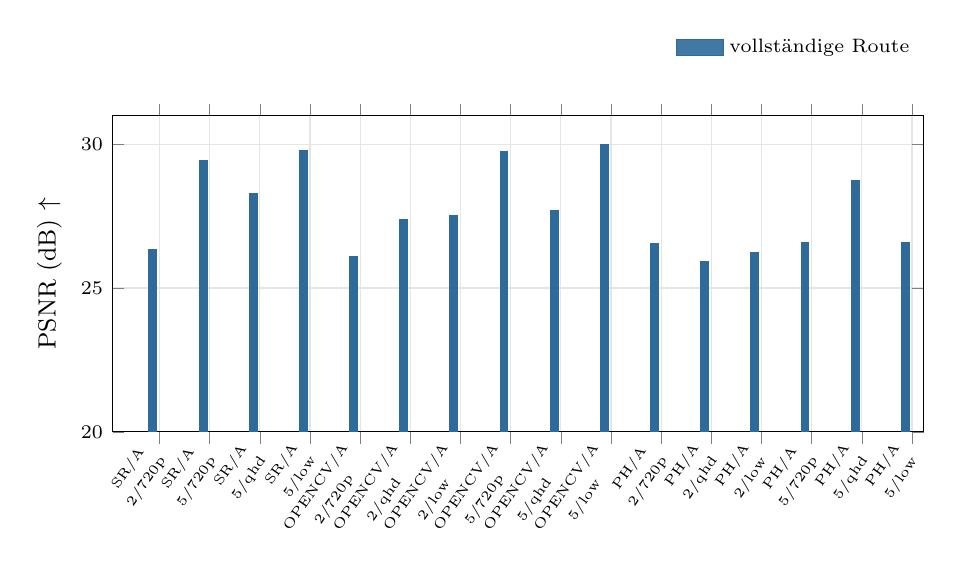
\begin{tikzpicture}
\begin{axis}[height=5.6cm,width=0.98\linewidth,ybar,bar width=2.8pt,enlarge x limits=0.015,xmin=-0.7,ymin=20,ymax=31,xtick=data,xticklabels={{\shortstack{SR/A\\2/720p}},{\shortstack{SR/A\\5/720p}},{\shortstack{SR/A\\5/qhd}},{\shortstack{SR/A\\5/low}},{\shortstack{OPENCV/A\\2/720p}},{\shortstack{OPENCV/A\\2/qhd}},{\shortstack{OPENCV/A\\2/low}},{\shortstack{OPENCV/A\\5/720p}},{\shortstack{OPENCV/A\\5/qhd}},{\shortstack{OPENCV/A\\5/low}},{\shortstack{PH/A\\2/720p}},{\shortstack{PH/A\\2/qhd}},{\shortstack{PH/A\\2/low}},{\shortstack{PH/A\\5/720p}},{\shortstack{PH/A\\5/qhd}},{\shortstack{PH/A\\5/low}}},x tick label style={font=\tiny,rotate=55,anchor=east},ylabel style={font=\small},tick label style={font=\scriptsize},ylabel={PSNR (dB) $\uparrow$},grid=major,grid style={gray!20},legend style={font=\scriptsize,at={(1.0,1.15)},anchor=south east,draw=none,fill=white,fill opacity=0.9,text opacity=1},xtick={0,1,2,3,4,5,6,7,8,9,10,11,12,13,14,15}]
\addplot+[fill=srblue,draw=srblue,area legend] coordinates {(0,26.33820363) (1,29.41639448) (2,28.29924453) (3,29.78896627) (4,26.09251831) (5,27.36821420) (6,27.51974000) (7,29.75600052) (8,27.68839292) (9,29.99353907) (10,26.54214463) (11,25.91712114) (12,26.21822335) (13,26.57282792) (14,28.71943249) (15,26.59301839)};
\addlegendentry{vollständige Route}
\addplot+[fill=incompletegray,draw=incompletegray,area legend] coordinates {};
\addlegendentry{STS-Zwischenmetrik unvollständiger Route}
\end{axis}
\end{tikzpicture}
\par\vspace{2pt}
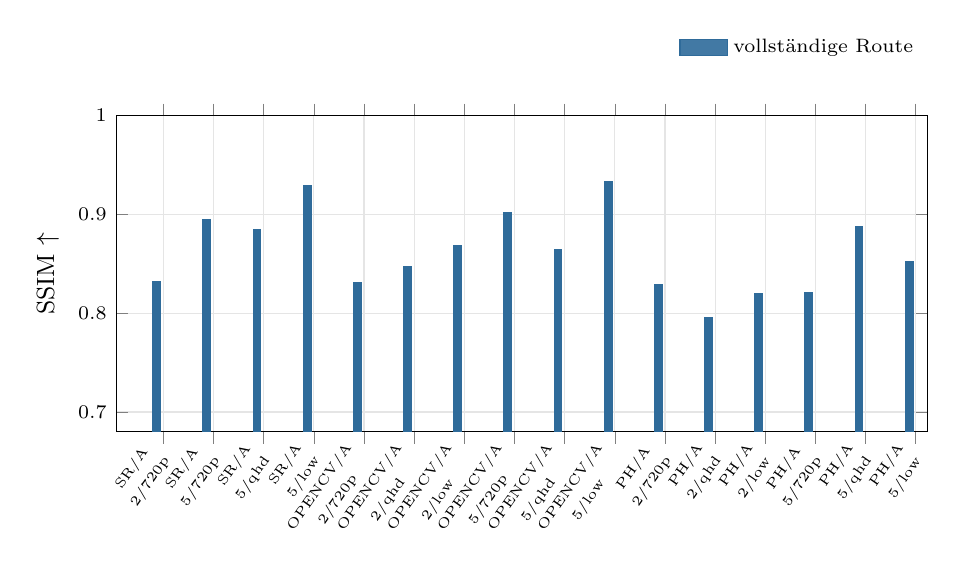
\begin{tikzpicture}
\begin{axis}[height=5.6cm,width=0.98\linewidth,ybar,bar width=2.8pt,enlarge x limits=0.015,xmin=-0.7,ymin=0.68,ymax=1.0,xtick=data,xticklabels={{\shortstack{SR/A\\2/720p}},{\shortstack{SR/A\\5/720p}},{\shortstack{SR/A\\5/qhd}},{\shortstack{SR/A\\5/low}},{\shortstack{OPENCV/A\\2/720p}},{\shortstack{OPENCV/A\\2/qhd}},{\shortstack{OPENCV/A\\2/low}},{\shortstack{OPENCV/A\\5/720p}},{\shortstack{OPENCV/A\\5/qhd}},{\shortstack{OPENCV/A\\5/low}},{\shortstack{PH/A\\2/720p}},{\shortstack{PH/A\\2/qhd}},{\shortstack{PH/A\\2/low}},{\shortstack{PH/A\\5/720p}},{\shortstack{PH/A\\5/qhd}},{\shortstack{PH/A\\5/low}}},x tick label style={font=\tiny,rotate=55,anchor=east},ylabel style={font=\small},tick label style={font=\scriptsize},ylabel={SSIM $\uparrow$},grid=major,grid style={gray!20},legend style={font=\scriptsize,at={(1.0,1.15)},anchor=south east,draw=none,fill=white,fill opacity=0.9,text opacity=1},xtick={0,1,2,3,4,5,6,7,8,9,10,11,12,13,14,15}]
\addplot+[fill=srblue,draw=srblue,area legend] coordinates {(0,0.83195574) (1,0.89474248) (2,0.88487382) (3,0.92957129) (4,0.83093130) (5,0.84708937) (6,0.86803825) (7,0.90132959) (8,0.86479931) (9,0.93359960) (10,0.82856342) (11,0.79535064) (12,0.81985135) (13,0.82038200) (14,0.88779274) (15,0.85198560)};
\addlegendentry{vollständige Route}
\addplot+[fill=incompletegray,draw=incompletegray,area legend] coordinates {};
\addlegendentry{STS-Zwischenmetrik unvollständiger Route}
\end{axis}
\end{tikzpicture}
\par\vspace{2pt}
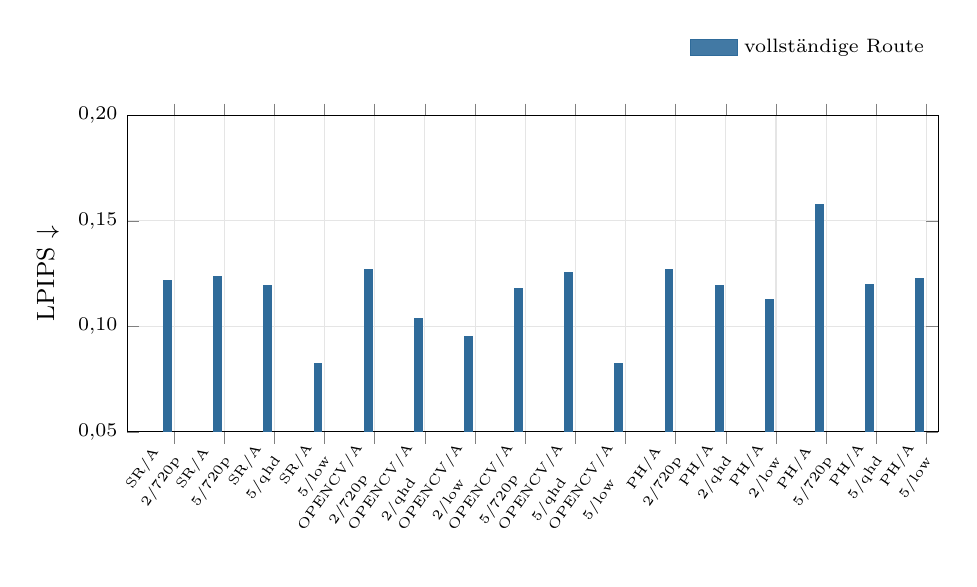
\begin{tikzpicture}
\begin{axis}[height=5.6cm,width=0.98\linewidth,ybar,bar width=2.8pt,enlarge x limits=0.015,xmin=-0.7,ymin=0.05,ymax=0.2,xtick=data,xticklabels={{\shortstack{SR/A\\2/720p}},{\shortstack{SR/A\\5/720p}},{\shortstack{SR/A\\5/qhd}},{\shortstack{SR/A\\5/low}},{\shortstack{OPENCV/A\\2/720p}},{\shortstack{OPENCV/A\\2/qhd}},{\shortstack{OPENCV/A\\2/low}},{\shortstack{OPENCV/A\\5/720p}},{\shortstack{OPENCV/A\\5/qhd}},{\shortstack{OPENCV/A\\5/low}},{\shortstack{PH/A\\2/720p}},{\shortstack{PH/A\\2/qhd}},{\shortstack{PH/A\\2/low}},{\shortstack{PH/A\\5/720p}},{\shortstack{PH/A\\5/qhd}},{\shortstack{PH/A\\5/low}}},x tick label style={font=\tiny,rotate=55,anchor=east},ylabel style={font=\small},tick label style={font=\scriptsize},ylabel={LPIPS $\downarrow$},grid=major,grid style={gray!20},scaled y ticks=false,ytick={0.05,0.10,0.15,0.20},yticklabels={{0,05},{0,10},{0,15},{0,20}},legend style={font=\scriptsize,at={(1.0,1.15)},anchor=south east,draw=none,fill=white,fill opacity=0.9,text opacity=1},xtick={0,1,2,3,4,5,6,7,8,9,10,11,12,13,14,15}]
\addplot+[fill=srblue,draw=srblue,area legend] coordinates {(0,0.12186836) (1,0.12371773) (2,0.11927220) (3,0.08216407) (4,0.12672276) (5,0.10358845) (6,0.09497066) (7,0.11802495) (8,0.12551100) (9,0.08218506) (10,0.12690219) (11,0.11930196) (12,0.11265756) (13,0.15761947) (14,0.11964402) (15,0.12276925)};
\addlegendentry{vollständige Route}
\addplot+[fill=incompletegray,draw=incompletegray,area legend] coordinates {};
\addlegendentry{STS-Zwischenmetrik unvollständiger Route}
\end{axis}
\end{tikzpicture}
\par\vspace{2pt}
\vspace{3pt}
\begin{minipage}{0.98\linewidth}\scriptsize Dargestellt werden ausschließlich vollständige Original-GS-A-Routen. Vorhandene \texttt{sts\_masked.json}-Dateien aus später fehlgeschlagenen SuGaR-Routen bleiben als Fehlernachweis archiviert, werden hier aber nicht zusätzlich dargestellt. Die Auswertung ist objektmaskiert; die Werte stammen aus der jeweiligen Runauflösung.\end{minipage}
\end{center}
\end{document}